\documentclass[12pt, notitlepage]{article}
%\usepackage[backend=biber]{biblatex}
\usepackage{amsmath}
\usepackage{listings}
\usepackage{graphicx}
\usepackage{caption}
%\usepackage{subcaption}
\usepackage{commath}
\usepackage{hyperref}
\usepackage{url}
\usepackage{xcolor}
\usepackage{textcomp}
\usepackage{dirtytalk}
\usepackage{listings}
\usepackage{wasysym}
\usepackage{float}
\usepackage{listings}
\usepackage[linesnumbered,lined,boxed,commentsnumbered]{algorithm2e}
\usepackage{subfig}

% Packages from derivations_fullproblem.tex
\usepackage[squaren]{SIunits}
\usepackage{a4wide}
\usepackage{array}
\usepackage{cancel}
\usepackage{amsmath}
\usepackage{amsfonts}
\usepackage{amssymb}
\usepackage{graphicx}
\usepackage{enumerate}
\usepackage{titling}

% Parameters for displaying code.
\lstset{language=python}
\lstset{basicstyle=\ttfamily\small}
\lstset{frame=single}
\lstset{keywordstyle=\color{red}\bfseries}
\lstset{commentstyle=\itshape\color{blue}}
\lstset{showspaces=false}
\lstset{showstringspaces=false}
\lstset{showtabs=false}
\lstset{breaklines}

% Define new commands
\newcommand{\expect}[1]{\langle #1 \rangle}
\newcommand{\dd}[1]{\ \text{d}#1}
\newcommand{\f}[2]{\frac{#1}{#2}} 
\newcommand{\tf}[2]{\tfrac{#1}{#2}}
\newcommand{\beq}{\begin{equation*}}
\newcommand{\eeq}{\end{equation*}}
\newcommand{\bra}[1]{\langle #1|}
\newcommand{\ket}[1]{|#1 \rangle}
\newcommand{\braket}[2]{\langle #1 | #2 \rangle}
\newcommand{\av}[1]{\left| #1 \right|}
\newcommand{\op}[1]{\widehat{#1}}
\newcommand{\braopket}[3]{\langle #1 | \op{#2} | #3 \rangle}
\newcommand{\ketbra}[2]{\ket{#1}\bra{#2}}
\newcommand{\pp}[1]{\frac{\partial}{\partial #1}}
\newcommand{\ppn}[1]{\frac{\partial^2}{\partial #1^2}}
\newcommand{\up}{\left|\uparrow\rangle\right.}
\newcommand{\down}{\left|\downarrow\rangle\right.}
\newcommand{\updown}{\left|\uparrow\downarrow\rangle\right.}
\newcommand{\downup}{\left|\downarrow\uparrow\rangle\right.}
\newcommand{\ua}{\uparrow}
\newcommand{\da}{\downarrow}
% Add bibliography
\begin{document}


\title{Summary - Classifying Events in Scintillator Data with Pre-Trained Neural Networks}
\author{Geir Tore Ulvik}
\maketitle
\section{Introduction}
A short summary of current work on using pre-trained neural networks to classify
single and double events in scintillator data.

\section{What are pre-trained networks and how do we use them?}
As the name suggests a pre-trained network is a network that has already
been trained, usually on very large amounts of data over a significant amount
of time. This is the case for the networks explored in this work. The networks
have all been trained on the "ImageNet" database and are on the cutting edge in
computer vision. They have also been analyzed extensively, increasing the amount
of insight in the learning process.

But we're not interested in classifying ImageNet data, we have our own data,
so how can we use the power of these networks for our own purposes?
The answer is \textbf{feature extraction}. When feeding an image forward
through the trained network, the various filters (or "kernels") react to different features
of the image, like edges or lines, general shapes etc. What we end up with on the other side
of the network is a "feature representation" of the input image. Hopefully, an input image
of say a cat and a car will produce significantly different feature representations, allowing
for classification. In our case we desire that the feature representations for single and
double events are different. This is the first thing we test when looking at which networks
might work for us.

\section{Data preparation}
In order to use the pre-trained networks, our data needs to be prepared to fit some requirements.
Additionally, the data was intentionally balanced such that the subset of 200000 events take from
the full dataset contained an equal amount of single and double events.
\subsection{Shape and Size}
The pre-trained networks are trained on RGB color images with a shape of $(224, 224, 3)$
corresponding to $(p_x, p_y, channels)$. Our data is much smaller, $(16, 16, 1)$. 
We solve the number of channels by concatenating our image data to itself, giving us 3 identical channels. 
Additionally, for the networks to accept our data we need to replace the input layer of each network,
with one that accepts our image size.
\subsection{Normalization of pixel values}
To reduce the risk of exploding and/or vanishing gradients, pixel values are commonly
normalized to $[0, 1]$ or to $[-1, 1]$ (with zero-mean). Here we have opted for a min-max scaling to the $[0, 1]$ interval.
The minimum and maximum pixel values are fetched for the entire dataset, such that intensity differences
between images are preserved. Min-max scaling is calculated as
\begin{equation}
    \text{scaled image} = \f{\text{image} - \mu_{image}}{I_{max} - I_{min}},
\end{equation}
where $I_{max}$ and $I_{min}$ refer to the maximum and minimum pixel intensity for the dataset,
and $\mu_{image}$ is the mean pixel intensity for the dataset. This scaling also preserves the
shape of the intensity distribution.

\section{Framework}
\begin{itemize}
    \item Python3
    \item TensorFlow (with Keras API)
    \item Scikit-Learn
    \item SciPy
\end{itemize}
\section{Networks}
The following networks have been explored to some degree.
\begin{itemize}
    \item DenseNet\{121, 169, 201\}
    \item InceptionResNetV2
    \item InceptionV3
    \item MobileNet
    \item MobileNetV2
    \item NASNetLarge
    \item NASNetMobile
    \item ResNet50
    \item VGG16
    \item VGG19
    \item Xception
\end{itemize}
\section{Feature Extraction}
To compare the extracted feature representations and find out if they may allow for classification,
a Kolmogorov-Smirnov(KS) two-sample test was performed. The test compares each feature's distribution
for single events and double events. The same test is also performed for single events and double events 
where the relative distance between events is $< 3mm$. The output p-value of the KS two-sample test
indicates whether or not we can reject the null hypothesis. The null hypothesis for one feature in this 
case is that for both single and double events the feature is drawn from the same underlying distribution.
For p-values lower than 0.01 we can generally reject the null-hypothesis. 

However, keep in mind that even if the feature distributions are different it's not a guarantee that 
classification will work. It is a necessary criterion, but not sufficient.
\subsection{Results}
The tables \ref{tab:features} and \ref{tab:features-close} show the number of features for each network,
and the ratio of features that have a p-value below certain thresholds corresponding to different levels
of significance. From the results it would seem that MobileNet and the NASNet variants may perform worse
than the rest of the networks, and VGG16 and VGG19 may follow the same trend. At the very least it seems
reasonable to bring each network with us in the next stages. We could perhaps discard MobileNet, but it
could be useful to keep as a sort of benchmark. We also don't know how many features need to be different
in order to make classification possible, and while the ratios for MobileNet are low, there's still
$0.227\cdot 2048 ~ 465$ different features, which is actually more features than MobileNetV2 and the Inception 
variants. Table \ref{tab:features-close} show only a slight decrease from \ref{tab:features}, so we will not
discard the possibility of classifying double events that are separated by only a small distance.
\begin{table}[h]
    \begin{tabular}{l|c|r|r|r}
	\hline
	 Network           &   features &   ratio $p < 0.01$ &   ratio $p < 0.005$ &   ratio $p < 0.001$ \\
	\hline
	 DenseNet121       &            512 &         1.00  &          1.00   &          1.00   \\
	 DenseNet169       &            512 &         1.00  &          1.00   &          1.00   \\
	 DenseNet201       &            512 &         1.00  &          1.00   &          1.00   \\
	 InceptionResNetV2 &            320 &         0.969 &          0.969  &          0.966  \\
	 InceptionV3       &            320 &         0.981 &          0.981  &          0.981  \\
	 MobileNet         &           2048 &         0.227 &          0.227  &          0.227  \\
	 MobileNetV2       &            384 &         1.00  &          1.00   &          1.00   \\
	 NASNetLarge       &           2058 &         0.510 &          0.510  &          0.510  \\
	 NASNetMobile      &            539 &         0.510 &          0.510  &          0.510  \\
	 ResNet50          &           4096 &         1.00  &          1.00   &          1.00   \\
	 VGG16             &            512 &         0.633 &          0.633  &          0.627  \\
	 VGG19             &            512 &         0.652 &          0.652  &          0.652  \\
	 Xception          &           3200 &         1.00  &          1.00   &          1.00   \\
	\hline
    \end{tabular}
    \caption{Comparison of feature distributions for single events and double events for all networks.
    The dataset is balanced, containing 100000 of each event type.}
    \label{tab:features}
\end{table}[h]
\begin{table}
    \begin{tabular}{lrrrr}
	\hline
	 Network           &   features &   ratio $p < 0.01$ &   ratio $p < 0.005$ &   ratio $p < 0.001$ \\
	\hline
	 DenseNet121       &            512 &         1.00  &          1.00  &          1.00  \\
	 DenseNet169       &            512 &         0.998 &          0.998 &          0.998 \\
	 DenseNet201       &            512 &         1.00  &          1.00  &          1.00  \\
	 InceptionResNetV2 &            320 &         0.969 &          0.969 &          0.966 \\
	 InceptionV3       &            320 &         0.972 &          0.969 &          0.962 \\
	 MobileNet         &           2048 &         0.222 &          0.221 &          0.219 \\
	 MobileNetV2       &            384 &         1.00  &          1.00  &          1.00  \\
	 NASNetLarge       &           2058 &         0.481 &          0.474 &          0.457 \\
	 NASNetMobile      &            539 &         0.458 &          0.445 &          0.419 \\
	 ResNet50          &           4096 &         1.00  &          0.999 &          0.999 \\
	 VGG16             &            512 &         0.602 &          0.599 &          0.598 \\
	 VGG19             &            512 &         0.643 &          0.643 &          0.639 \\
	 Xception          &           3200 &         1.00  &          1.00  &          0.999 \\
	\hline
    \end{tabular}
    \caption{Comparison of feature distributions for single events and double events with relative distance
	between events $< 3mm$. The dataset contain 100000 single events and 11006 double events.}
    \label{tab:features-close}
\end{table}

\section{A closer look at the data}
One of the challenges with this classification task is to correctly classify double events that
are separated by small distances ($< 3mm$). These are events that are difficult even for
humans to correctly classify. In figure \label{fig:relative-all} the distribution of relative
distances and relative energy differences for all double events in the dataset are shown.
\begin{figure}
    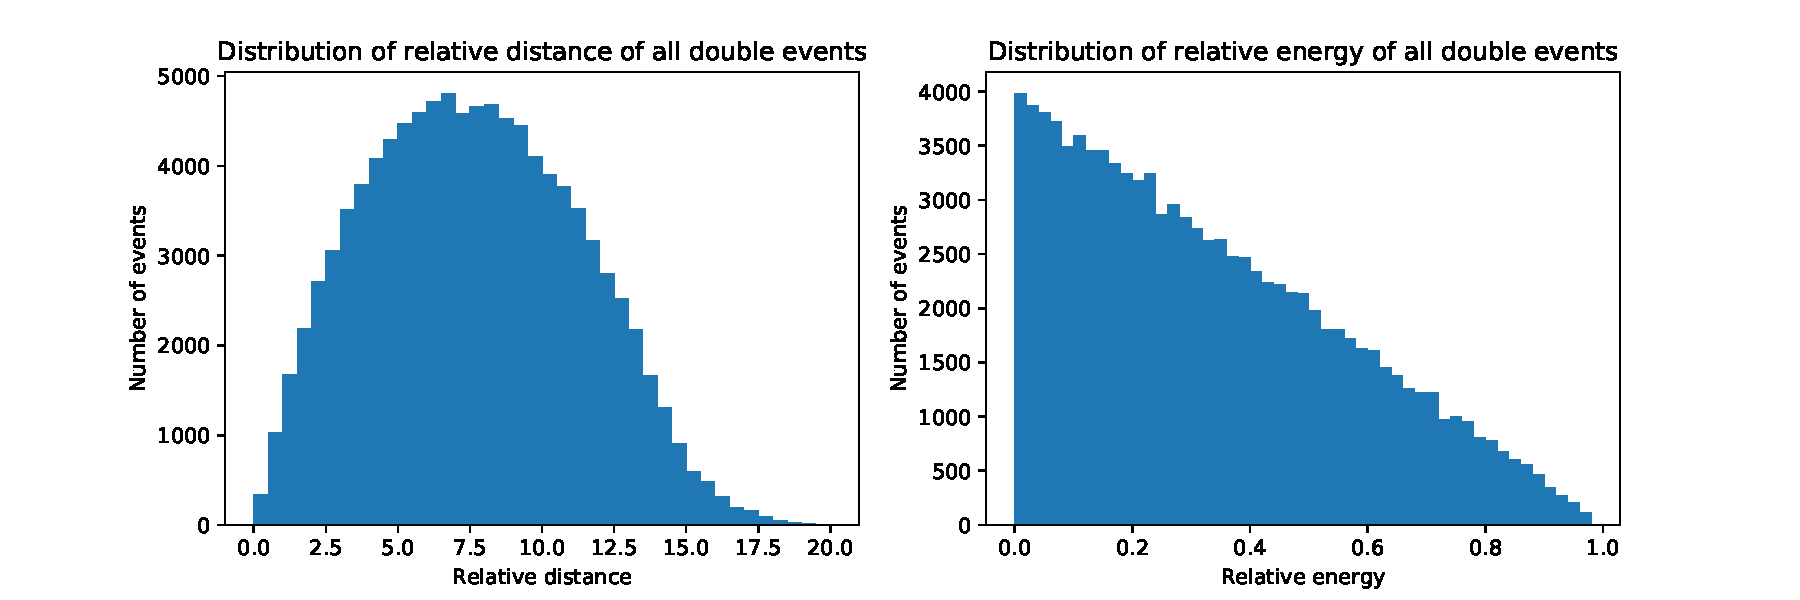
\includegraphics[width=\textwidth]{figures/DenseNet201_relative_all}
    \caption{Distributions of relative distances and energies for all double events in the dataset
    of 200000 events. Each bin in the left plot is $0.5mm$ wide, while the width of bins in the
    right plot is $0.02$. $\mu_{distance}=7.65mm$, $\mu_{energy}=0.33$.}
    \label{fig:relative-all}
\end{figure}
From figure \ref{fig:relative-all} we see that the relative distances individual events of a
double event are close to a gaussian disitribution, while the relative energies are linearly
distrubuted, decreasing in number of events with increasing energy difference.
From figure \ref{fig:relative-test} we can see that the test set, selected after shuffling the
dataset, follows the same distribution.
\begin{figure}
    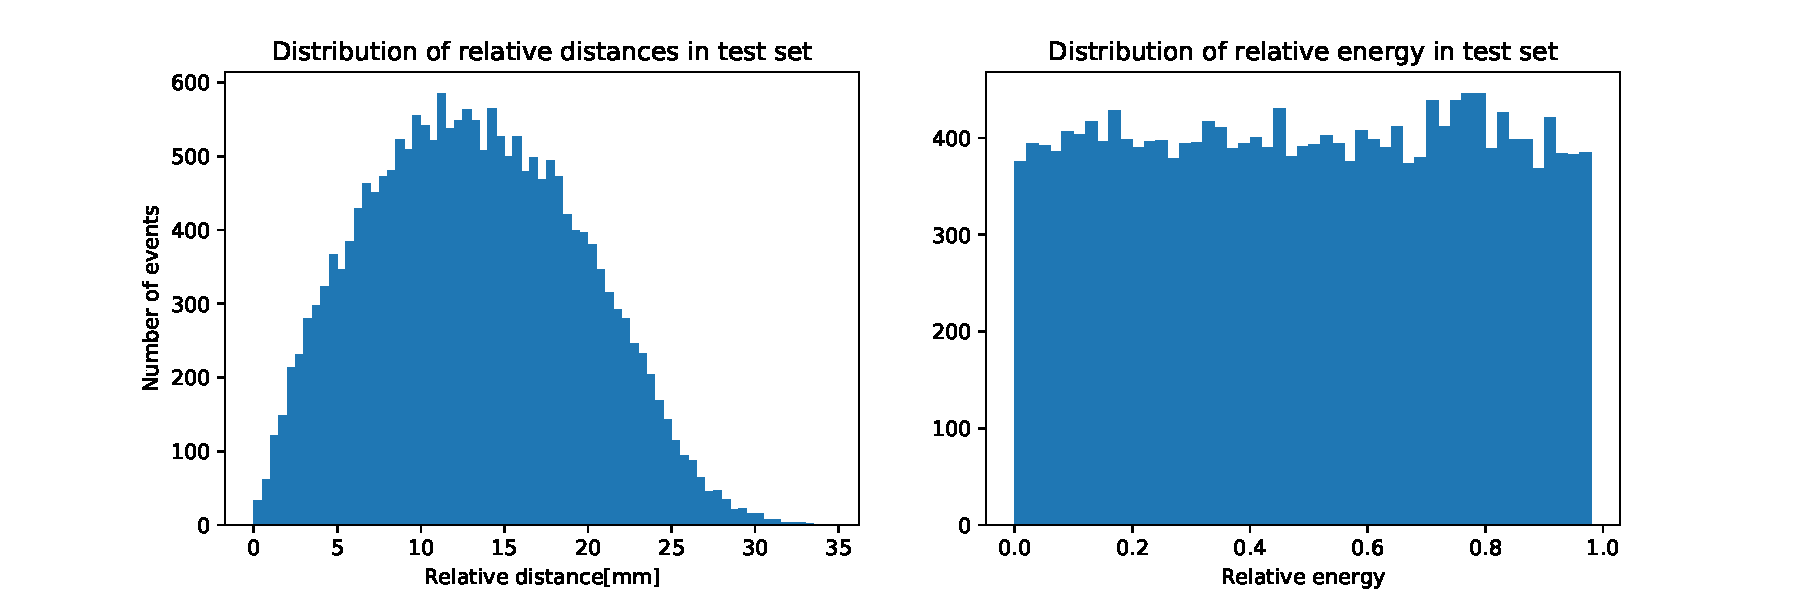
\includegraphics[width=\textwidth]{figures/DenseNet201_relative_test}
    \caption{Distributions of relative distances and energies for double events in the test set. 
    Each bin in the left plot is $0.5mm$ wide, while the width of bins in the
    right plot is $0.02$. $\mu_{distance}=7.64mm$, $\mu_{energy}=0.33$.}
    \label{fig:relative-all}
\end{figure}
From this we might expect the models to be worse at classifying double events with large relative
energy differences, and with small relative distances separating them. If the relative distance
is large it is visually very simple to see that it is a double event, but if the energy difference
is also very large, then one event might barely be visible. Additionaly, these are the types of events
that the model will see less of during training.

\section{Classification}
Classification was performed on the feature representations using K-Fold cross-validation.
This provides a better insight into how the model's performance varies with the data it's
trained on, and gives a more realisting view of performance.
The networks' results are presented in table \ref{tab:accuracies}.

\begin{table}[h]
    \begin{tabular}{l|r|r|r}
	Network           & Min Accuracy & Max Accuracy & Mean Accuracy \\
	\hline
	DenseNet121       & 0.92         & 0.93         & 0.92          \\
	DenseNet169       & 0.92         & 0.93         & 0.92          \\
	DenseNet201       & 0.92         & 0.94         & 0.93          \\
	InceptionResNetV2 & 0.88         & 0.89         & 0.88          \\
	InceptionV3       & 0.87         & 0.88         & 0.88          \\
	MobileNet         & 0.50         & 0.86         & 0.71          \\
	MobileNetV2       & 0.50         & 0.50         & 0.50          \\
	NASNetLarge       & 0.91         & 0.92         & 0.92          \\
	NASNetMobile      & 0.91         & 0.92         & 0.92          \\
	ResNet50          & 0.50         & 0.50         & 0.50          \\
	VGG16             & 0.91         & 0.92         & 0.91          \\
	VGG19             & 0.88         & 0.90         & 0.89          \\
	Xception          & 0.92         & 0.93         & 0.92         
    \end{tabular}
    \caption{Table of accuracy scores for all pretrained networks after K-Fold cross-validation
    with five folds. Minimum, maximum, and mean accuracy score for all networks.}
    \label{tab:accuracies}
\end{table}

\subsection{DenseNet201}
To explore the classification results further we explore the highest scoring model, DenseNet201.
We load instance of DenseNet201 which performed at an accuracy of 0.94. When assessing the
performance of the model, it is useful to know not only how many events were classified correctly,
but also what was classified wrong. To see this we plot the confusion matrix, presented in figure
\ref{fig:DN201-confusion-matrix}.
\begin{figure}
    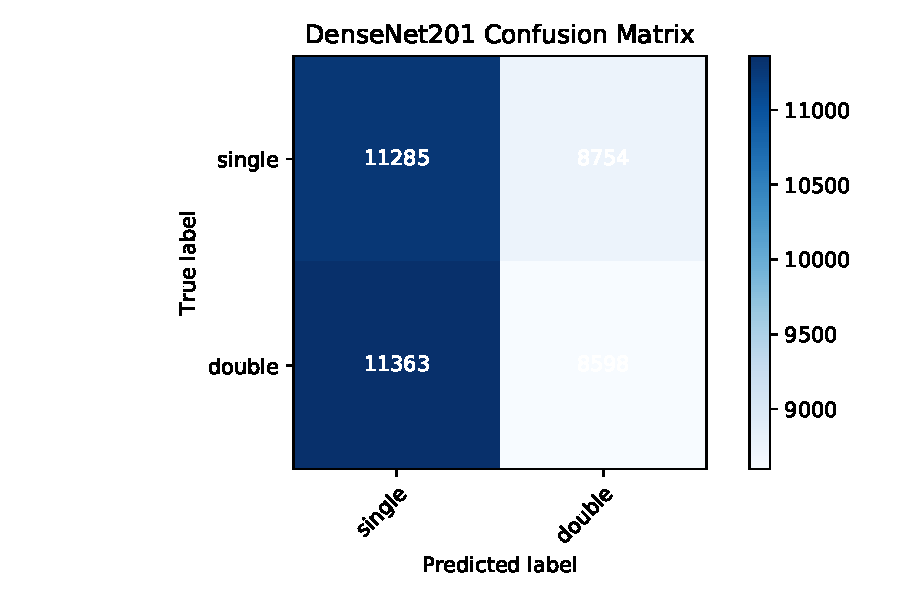
\includegraphics[width=\textwidth]{figures/DenseNet201_confmat}
    \caption{Confusion matrix for DenseNet201. Ratio of correct single events is 0.99, and ratio
    of correct double events is 0.89. For events separated by a distance $< 3mm$ the ratio is 0.63.}
    \label{fig:DN201-confusion-matrix}
\end{figure}
From the confusion matrix, and the classification ratios ($r_{single}=0.99$, $r_{double}=0.89$, $r_{close}=0.63$),
we can see that the model is very good at classifying single events, and fairly good at double events in general.
Very few single events are classified as double events. There are, however, a fair number of double events that
are classified as single events. To provide another view of the classification results we plot the distributions
of relative distances and relative energies for the predictions, separated into correct and wrong classifications
in figure \ref{fig:relative-compare}. Combining these results makes it clear that the model struggles the most with double
events that are close together.
\begin{figure}
    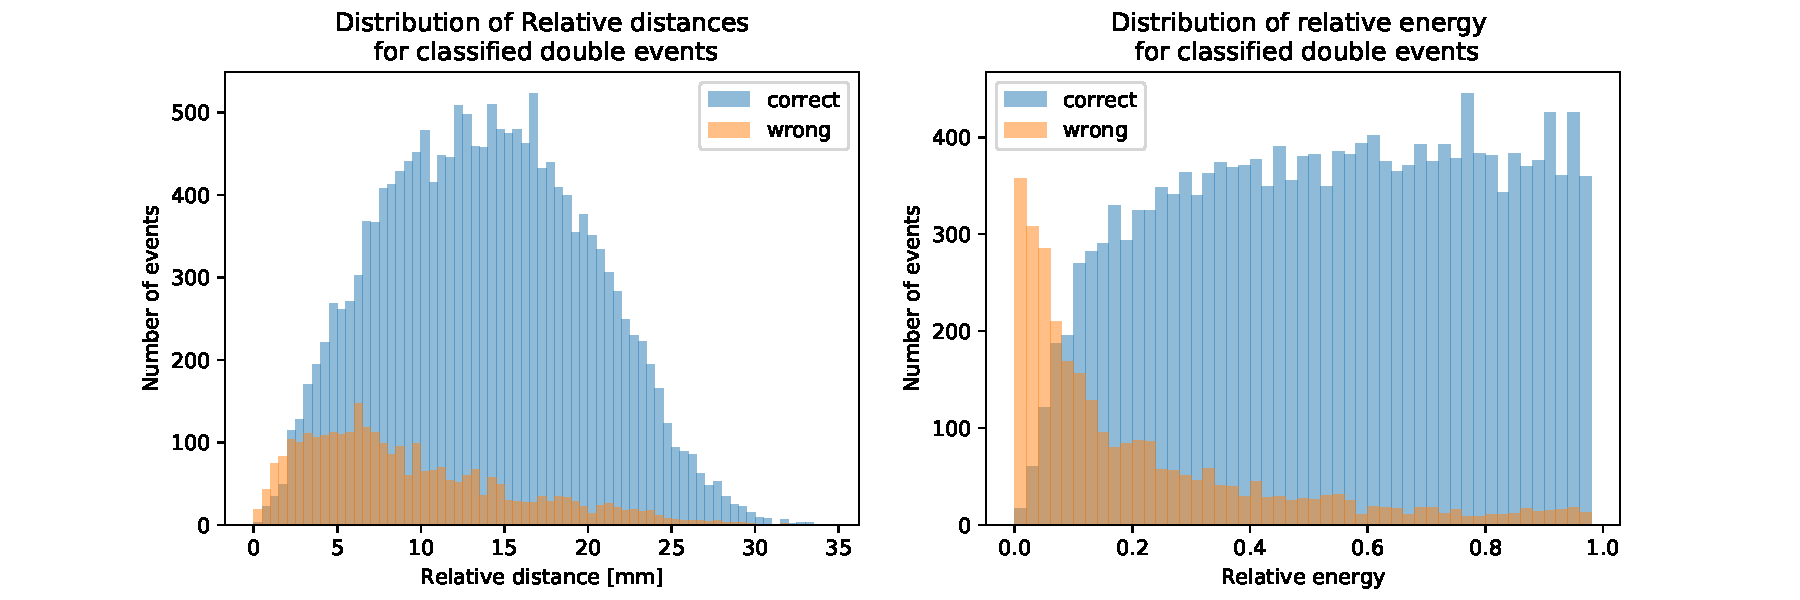
\includegraphics[width=\textwidth]{figures/DenseNet201_relative_test_compare}
    \caption{Distributions of relative distances and relative energies for classified double events,
    separated into events that were correctly classified, and events that were classified wrong.}
    \label{fig:relative-compare}
\end{figure}

\subsection{Difficult Events}
The results above show that double events separated by small distances are indeed the 'difficult' events.
But are they difficult for all the models? To verify if this is the case, events that were not classified
correctly were stored for each network during evaluation. We then took the intersect of the set of unique
events for each network, resulting in 356 events that none of the networks were able to classify correctly.
For comparison, the number of close double events is 2181. In figure \ref{fig:relative-noncorrect} we show
the distributions for distances and energies for these 'never correct' events.
\begin{figure}
    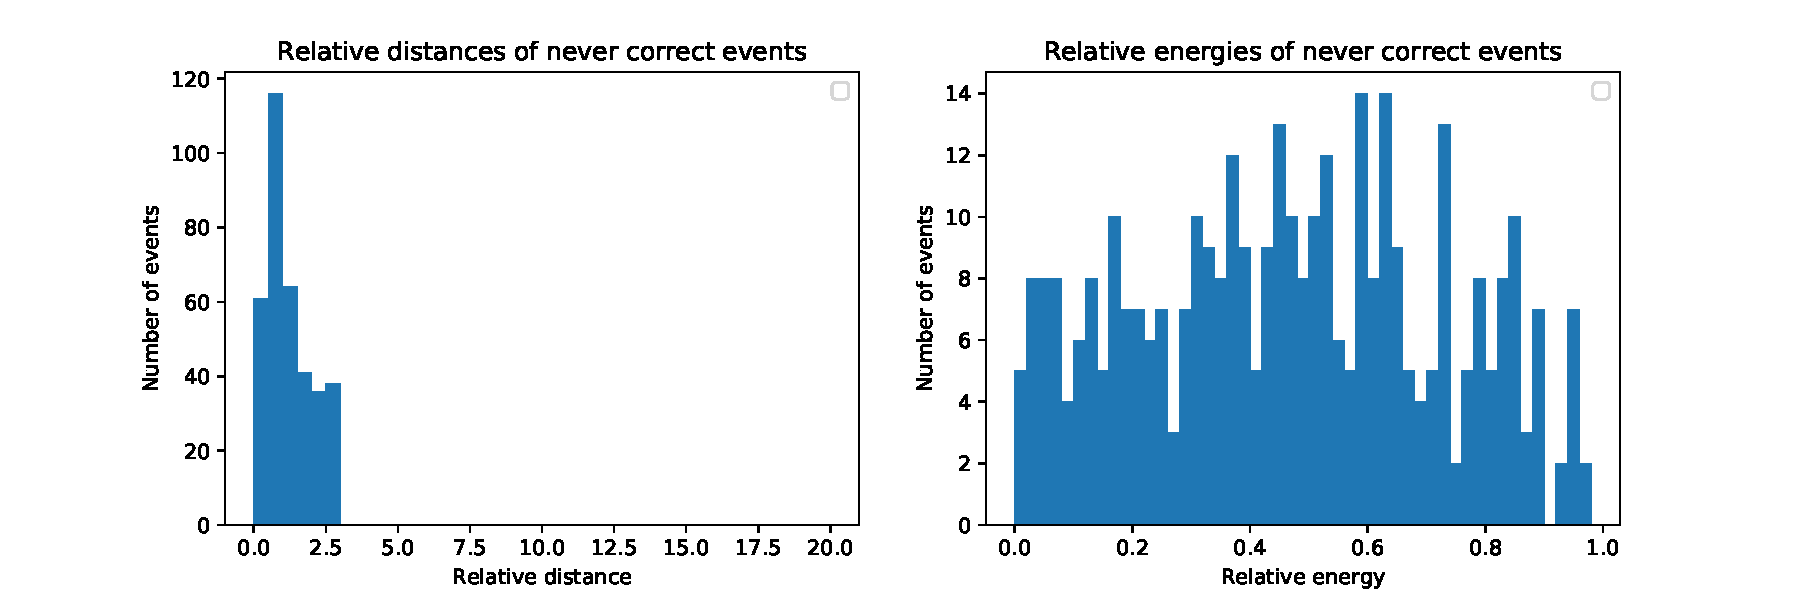
\includegraphics[width=\textwidth]{figures/DenseNet201_relative_noncorrect}
    \caption{Distributions of relative distances and relative energies for classified double events,
    separated into events that were correctly classified, and events that were classified wrong.}
    \label{fig:relative-noncorrect}
\end{figure}
The distribution of relative distances further solidify that close events are the most difficult ones.
It would also seem that the relative energy difference doesn't have a large impact on classification
accuracy, at least not for the difficult events. The trend of a rising amount of wrong classifications with
increasing relative energy difference, as seen in figure \ref{fig:relative-compare}, could be attributed
to the decreasing amount of samples seen during training. A selection of images of difficult events
can be seen in figure \ref{fig:nocorrect-samples}.
\begin{figure}
    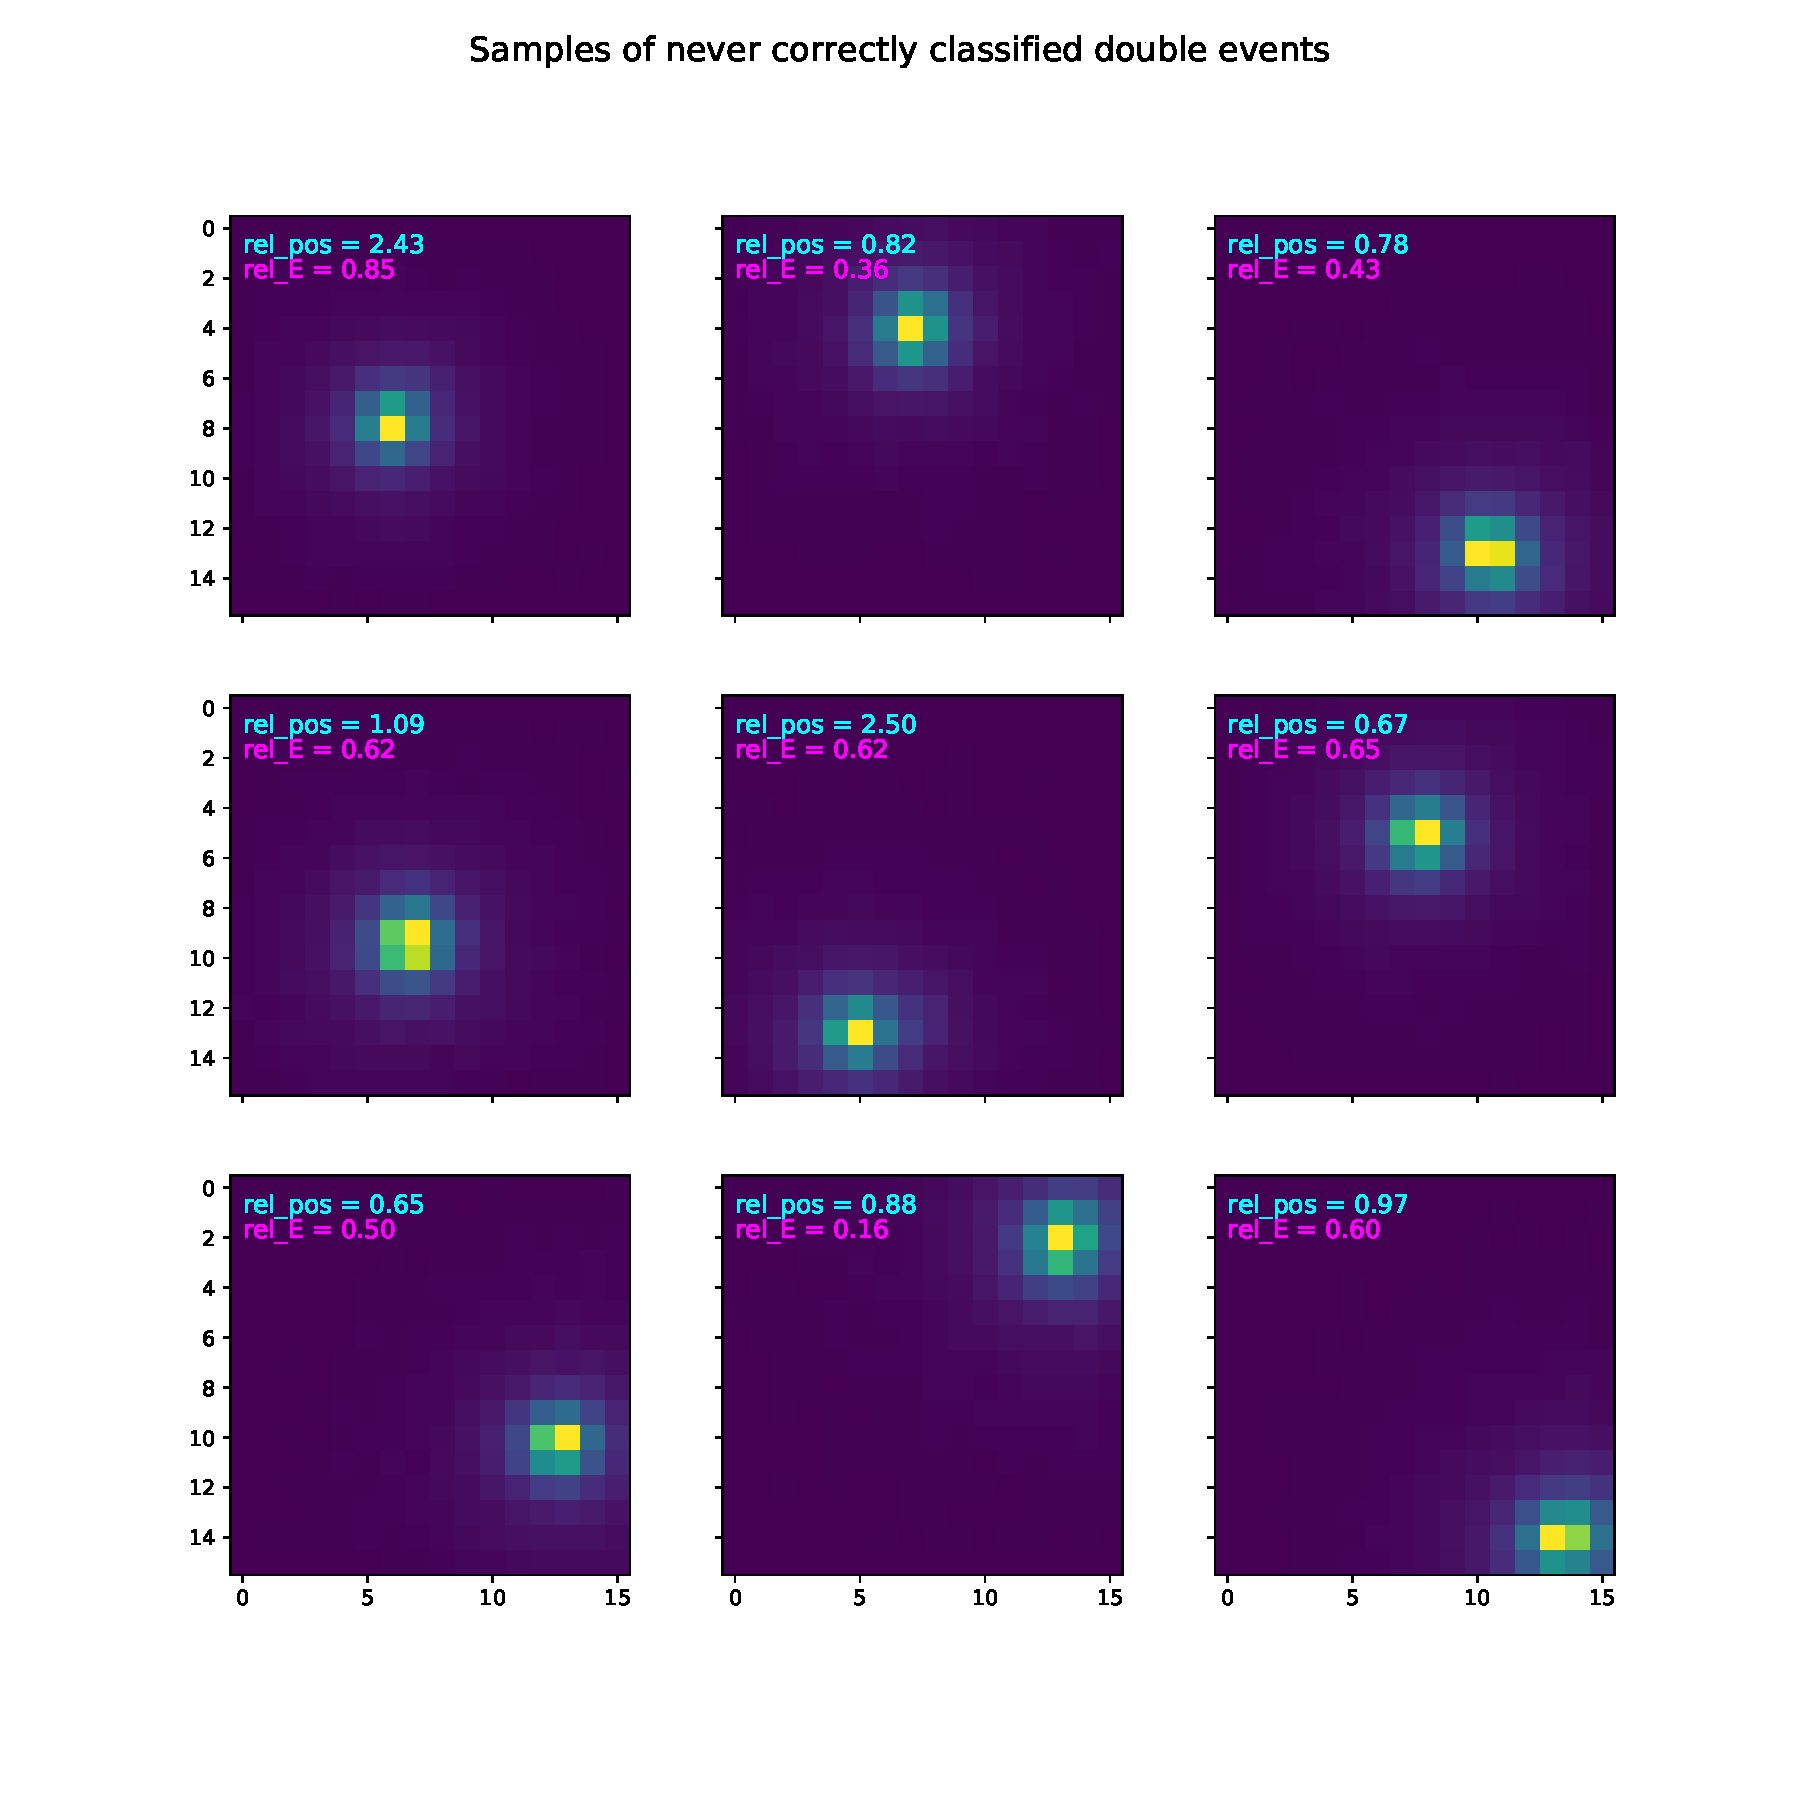
\includegraphics[width=\textwidth]{figures/DenseNet201_nocorrect_samples}
    \caption{Selected images of difficult events. rel\_dist is the relative distance between
    the events in the image, and rel\_E is the relative energy difference.}
    \label{fig:nocorrect-samples}
\end{figure}

%\appendix
%\bibliographystyle{unsrt}
%\bibliography{bibliography}
\end{document}


% Result from new run of feature distribution comparisons
%\begin{tabular}{lrrrr}
%\hline
% Network           &   num\_features &   ratio p \ensuremath{<} 0.01 &   ratio p \ensuremath{<} 0.005 &   ratio p \ensuremath{<} 0.001 \\
%\hline
% DenseNet121       &            512 &         1        &          1        &          1        \\
% DenseNet169       &            512 &         1        &          1        &          1        \\
% DenseNet201       &            512 &         1        &          1        &          1        \\
% InceptionResNetV2 &            320 &         0.965625 &          0.965625 &          0.965625 \\
% InceptionV3       &            320 &         0.959375 &          0.959375 &          0.959375 \\
% MobileNet         &           2048 &         0.224609 &          0.224609 &          0.224121 \\
% MobileNetV2       &            384 &         1        &          1        &          1        \\
% NASNetLarge       &           2058 &         0.510204 &          0.510204 &          0.510204 \\
% NASNetMobile      &            539 &         0.510204 &          0.510204 &          0.510204 \\
% ResNet50  &           4096 &         1        &          1        &          1        \\
% VGG16     &            512 &         0.609375 &          0.607422 &          0.607422 \\
% VGG19     &            512 &         0.632812 &          0.630859 &          0.626953 \\
% Xception  &           3200 &         1        &          1        &          1        \\
%\hline
%\end{tabular}
